\documentclass[../tfg.tex]{subfiles}

\begin{document}

\section{The stack}
The most common way for CPUs to implement procedure or subroutine calls is by the means of a stack\cite{intel:1}. Thanks to its last-in first-out nature, the stack is a simple and effective solution to keep track of the order of the callings: \emph{when you call a subroutine, you push the address of the next instruction onto the stack and once the subroutine has finished executing you can return where you left by popping the previously pushed address.}
The address of the next instruction pushed on the stack is called the \textbf{return address}.
\\

\begin{minipage}[c]{0.4\linewidth}
\begin{lstlisting}
void do_something() {
    do_something_a();
    // 2
    do_something_b();
    // 3
}

int main() {
    do_something();
    // 1
    return 0;
}
\end{lstlisting}
\end{minipage}
\begin{minipage}[c]{0.6\linewidth}
    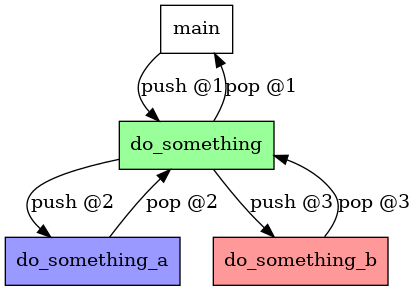
\includegraphics[width=\linewidth]{imgs/stack_overflows/simple_stack_graph.png}
\end{minipage}
\begin{figure}[H]
    \centering
    \subfile{../imgs/stack_overflows/simple_stack_timeline}
    \caption{Simplified stack timeline}
    \label{fig:simple_stack_timeline}
\end{figure}

This stack coexists in the main memory of the computer along the code and the data and for Intel x86 and x86\_64 CPUs, it is controlled by two registers: the \textbf{stack pointer} and the \textbf{base pointer}.

\subsection{Stack frame}

The stack holds much more information that just the execution path that the program has taken. It also holds local variables, the previous base pointer before the call and subroutine arguments and return values (it may vary between calling conventions).

To group all that data associated with a subroutine call, we use the term \textbf{stack frame}, and it is composed of the following components (in push order):
\begin{enumerate}
    \item Parameters of the subroutine. In 64-bit Linux, the default calling convention specifies that the first 5 parameters must be passed on registers instead of the stack.
    \item Return address.
    \item Locals of the subroutine.
\end{enumerate}

The stack drawed in Figure \ref{fig:c32_stack_layout} is an example of stack frame for the \texttt{foo} procedure.

\begin{figure}[H]
    \centering
    \subfile{../imgs/stack_overflows/c32_stack_layout}
    \caption{Standard C 32-bit calling convention stack layout}
    \label{fig:c32_stack_layout}
\end{figure}


\subsection{Overflowing the stack}
Now that we know that the stack contains a mix of modifiable variables and critical data like the return address comes an important question:
\begin{center}
\emph{Can we modify the return address?} \textbf{Indeed}.
\end{center}

Consider the following stack, Figure \ref{fig:stack_buffer}. It has a local variable called \texttt{buffer} that spans for $n$ bytes. If we fill that buffer with $n + 1$ bytes, the excess of $1$ byte will overwrite partially the saved base pointer (bp). To overwrite the return address we just need to fill the buffer with $n + \texttt{sizeof(bp)} + \texttt{sizeof(ip)}$ bytes.\\\\
When the processor finishes executing the subroutine, it will pop the return address and set the instruction pointer register to that value, \textbf{executing the bytes found at that address as code}. By choosing precise values for the return address we can redirect code execution wherever we want.


\begin{figure}[H]
    \centering
    \subfile{../imgs/stack_overflows/stack_buffer}
    \caption{Buffer on the stack}
    \label{fig:stack_buffer}
\end{figure}

\section{Basic overflow}
\label{stack_overflow:ret2win}
To do a basic stack overflow I recommend using a premade environment with all the protections disabled to focus on the basic exploit. For this first example, I will use the virtual machine \textit{Phoenix} found at \href{https://exploit.education}{\texttt{exploit.education}}, specifically the level \href{http://exploit.education/phoenix/stack-four/}{\textit{Stack4}}.

\begin{figure}[H]
    \centering
    \subfile{../imgs/stack_overflows/phoenix_stack4_code}
    \caption{Stack4@Phoenix}
    \label{fig:phoenix_stack4_code}
\end{figure}

On this level we found a \textbf{ret2win} exercise. The code contains a function \texttt{win} that is never called but is present on the binary. The goal is to execute that function overwriting the return address to point to the address of \texttt{win}. In order to achieve the stack overflow we need to input more data than expected so we can overflow the buffer on the stack and override the return address. There are a few functions in the C Standard Library that do not perform bounds checking on the input received: in this particular case, we are presented with the function \texttt{gets}. A quick look into the man page of that function reveals the vulnerability on the bugs section.

\begin{figure}[H]
    \centering
    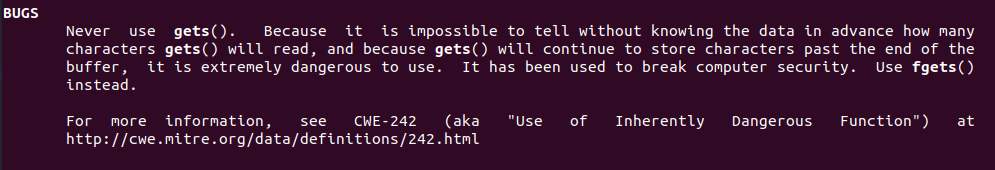
\includegraphics[width=\linewidth]{imgs/stack_overflows/man_gets_bugs.png}
    \caption{\texttt{man 3 gets}: Bugs section}
    \label{fig:man_gets_bugs}
\end{figure}


We need to supply \texttt{gets} with the following data:
\begin{enumerate}
\item $64$ bytes of junk for the buffer
\item $8$ bytes of junk for the \texttt{ret} local variable
\item $8$ bytes of junk for the stack alignment padding\cite{intel:1}
\item $8$ bytes of junk for the saved base pointer
\item $8$ bytes with the address of \texttt{complete\_level} for the return address
\end{enumerate}

To find the address of \texttt{complete\_level} we can use a debugger like \texttt{gdb}.

A simple Python 2.7 script will do the job.
\lstinputlisting[language=python, caption={stack4\_exploit.py}]{../../src/phoenix/stack4_exploit.py}

And we are done.

\begin{figure}[H]
    \centering
    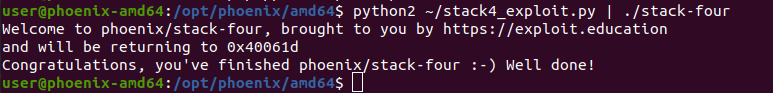
\includegraphics[width=\linewidth]{imgs/stack_overflows/phoenix_stack4_solved.png}
    \caption{Exploiting Stack4}
    \label{fig:phoenix_stack4_solved}
\end{figure}

Some last thoughts on why that exploit was possible:
\begin{itemize}
\item We knew in advance the address where \texttt{complete\_level} was loaded
\item No bounds checking was performed on the user input
\item There was nothing checking the integrity of the stack frame
\end{itemize}

\section{Shellcode injection}
In the last exploit we returned to the \texttt{win} function to solve the challenge. But in the general case we want to achieve \textbf{arbitrary code execution}, not just returning to the functions already present in the binary. This can be done by passing as input the machine code of the instructions we would like to execute and override the return address to point to wherever we store that machine code, thus injecting and executing the shellcode.
Take a look at the next exercise: \href{http://exploit.education/phoenix/stack-five/}{\textit{Stack5}} from the \textit{Phoenix} VM.

\begin{lstlisting}
/* ... */

void start_level() {
  char buffer[128];
  gets(buffer);
}

int main(int argc, char **argv) {
  printf("%s\n", BANNER);
  start_level();
}
\end{lstlisting}

The program is very similar to the \textit{Stack4}: a buffer on the stack and a call to \texttt{gets}, that we know is vulnerable to overflows. On the last exploit, almost all of our input was just junk bytes. In this exploit, we are going to use that junk space to store the shellcode and the return address will point to the start of the shellcode.

If the last exploit was called \textbf{ret2win} because we returned to the \texttt{win} function this exploit could be named \textbf{ret2stack} or \textbf{ret2buffer} because we will be returning to the buffer on the stack.

You could assemble your own shellcode manually, but I am going to use this shellcode found at \href{http://shell-storm.org/shellcode/files/shellcode-806.php}{\texttt{shell-storm.org}} that performs an \texttt{execve("/bin/sh")}.

The format of the input to \texttt{gets} will be:
\begin{enumerate}
    \item 27 bytes of shellcode
    \item $128 - len(shellcode)$ bytes of NOPs to fill the buffer
    \item 8 bytes of NOPs for the saved base pointer
    \item 8 bytes with the address of the start of the buffer, where our shellcode is located
\end{enumerate}

We will change the junk bytes with NOP opcodes (0x90) because we are now executing instructions on the stack. If the CPU starts executing and finds random bytes, it will launch an invalid opcode exception and kill the process. In this particular case it does not matter because the shellcode is at the beginning and the \texttt{execve} will replace the process image with the one from \texttt{/bin/sh}, including the stack but while you are debugging the shellcode and the exploit they can be essential.

In my \texttt{gdb} debugging session I found the address of the start of the buffer to be \texttt{0x7fffffffe490}, and so I plugged that number into my exploit script.
\begin{lstlisting}
exploit = "\x31\xc0\x48\xbb\xd1\x9d\x96\x91\xd0\x8c\x97\xff\x48"\
          "\xf7\xdb\x53\x54\x5f\x99\x52\x57\x54\x5e\xb0\x3b\x0f\x05"
exploit += "\x90" * (128 - len(exploit))
exploit += "\x90" * 8
exploit += "\x90\xe4\xff\xff\xff\x7f\x00\x00"
print exploit
\end{lstlisting}

Inside the debugger the script worked, but outside it failed. Taking a closer look into the error we can see that the value for the \texttt{rsp} register once we returned from \texttt{start\_level} is different from the value it had inside the debugger. This offset causes us to jump to a wrong address and instead of our shellcode the CPU is trying to execute random bytes and thus, provoking an illegal opcode trap. We have to account for that difference in our script.

\begin{figure}[H]
    \centering
    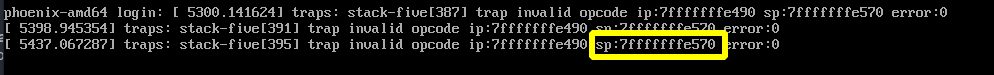
\includegraphics[width=\linewidth]{imgs/stack_overflows/stack5_wrong_return.png}
    \vspace{0.1cm}
%\end{figure}

%\begin{figure}[H]
%    \centering
    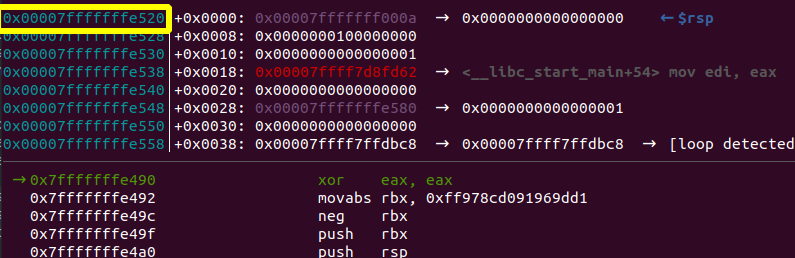
\includegraphics[width=\linewidth]{imgs/stack_overflows/stack5_wrong_return_gdb.png}
    \vspace{0.1cm}
%\end{figure}

%\begin{figure}[H]
%    \centering
    \subfile{../imgs/stack_overflows/stack5_stack_offset}
    \caption{Stack offsets between debugged process and non debugged process}
\end{figure}

$$ 0x...570 - 0x...520 = 0x50 $$

We have to add this offset to the start of the buffer, $0x...490$.

$$ 0x...490 + 0x50 = 0x...4e0 $$

This problem did not happen in the last challenge because we were not returning to the stack but to a function in the binary.

\lstinputlisting[language=python, caption={stack5\_exploit.py}]{../../src/phoenix/stack5_exploit.py}

\label{stack_overflows:shell_concatenate_stdin}
One last thing. The shell runs in interactive mode by default and it expects to be connected to \texttt{stdin}. If you do not redirect standard input to the shell, it will close automatically upon start, so you need to concatenate the python output with standard input and pass everything to the executable.

\begin{figure}[H]
    \centering
    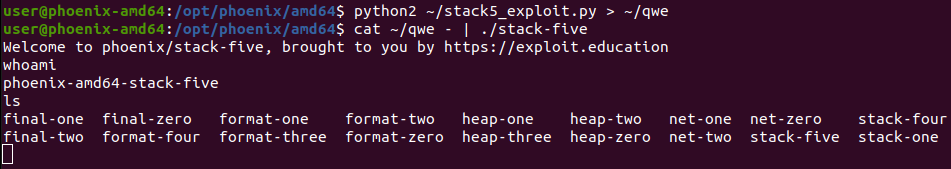
\includegraphics[width=\linewidth]{imgs/stack_overflows/stack5_solved.png}
\end{figure}

Some thoughts on why this exploit was possible:
\begin{itemize}
\item We knew in advance the address of the buffer on the stack.
\item No bounds checking was performed on the user input.
\item There was nothing checking the integrity of the stack frame.
\item We could execute instructions stored on the stack.
\end{itemize}

\end{document}
